\section{Introduction}

In connectomics, neuroscientists annotate neurons and their connectivity within 3D volumes to gain insight into the functional structure of the brain. Rapid progress in automatic sample preparation and electron microscopy (EM) acquisition techniques has made it possible to image large volumes of brain tissue at $\approx4\, nm$ per pixel to identify cells, synapses, and vesicles. For $40\, nm$ thick sections, a $1\, mm^3$ volume of brain contains $10^{15}$ voxels, or 1 petabyte of data. With so much data, manual annotation is infeasible, and automatic annotation methods are needed ~\cite{jain2010,Liu2014,GALA2014,kaynig2015large}.

Automatic annotation by segmentation and classification of brain tissue is challenging~\cite{isbi_challenge}. The state of the art uses supervised learning with convolutional neural networks~\cite{Ciresan:2012f}, or potentially even unsupervised learning~\cite{BogovicHJ13}. Typically, cell membranes are detected in 2D images, and the resulting region segmentation is grouped into geometrically-consistent cells across registered sections. Cells may also be segmented across registered sections in 3D directly. Using dynamic programming techniques~\cite{Masci:2013a} and a GPU cluster, these classifiers can segment $\approx1$ terabyte of data per hour ~\cite{kasthuri2015saturated}. This is sufficient to keep up with the 2D data capture process on state-of-the-art electron microscopes (though 3D registration is still an expensive offline operation).

All automatic methods make errors, and we are left with large data which needs \emph{proofreading} by humans. This crucial task serves two purposes: 1) to correct errors in the segmentation, and 2) to provide a large body of labeled data to train better automatic segmentation methods. Recent proofreading tools provide intuitive user interfaces to browse segmentation data in 2D and 3D and to identify and manually correct errors ~\cite{markus_proofreading,raveler,mojo2,haehn_dojo_2014}. Many kinds of errors exist, such as inaccurate boundaries, but the most common are \emph{split errors}, where a single segment is labeled as two, and \emph{merge errors}, where two segments are labeled as one (Fig.~\ref{fig:merge_and_slit_errors}). With user interaction, split errors can be joined, and the missing boundary in a merge error can be defined with manually-seeded watersheds~\cite{haehn_dojo_2014}. However, even with semi-automatic correction tools, the visual inspection to find errors in the first place takes the majority of the time.

\begin{figure}[t]
\begin{center}
  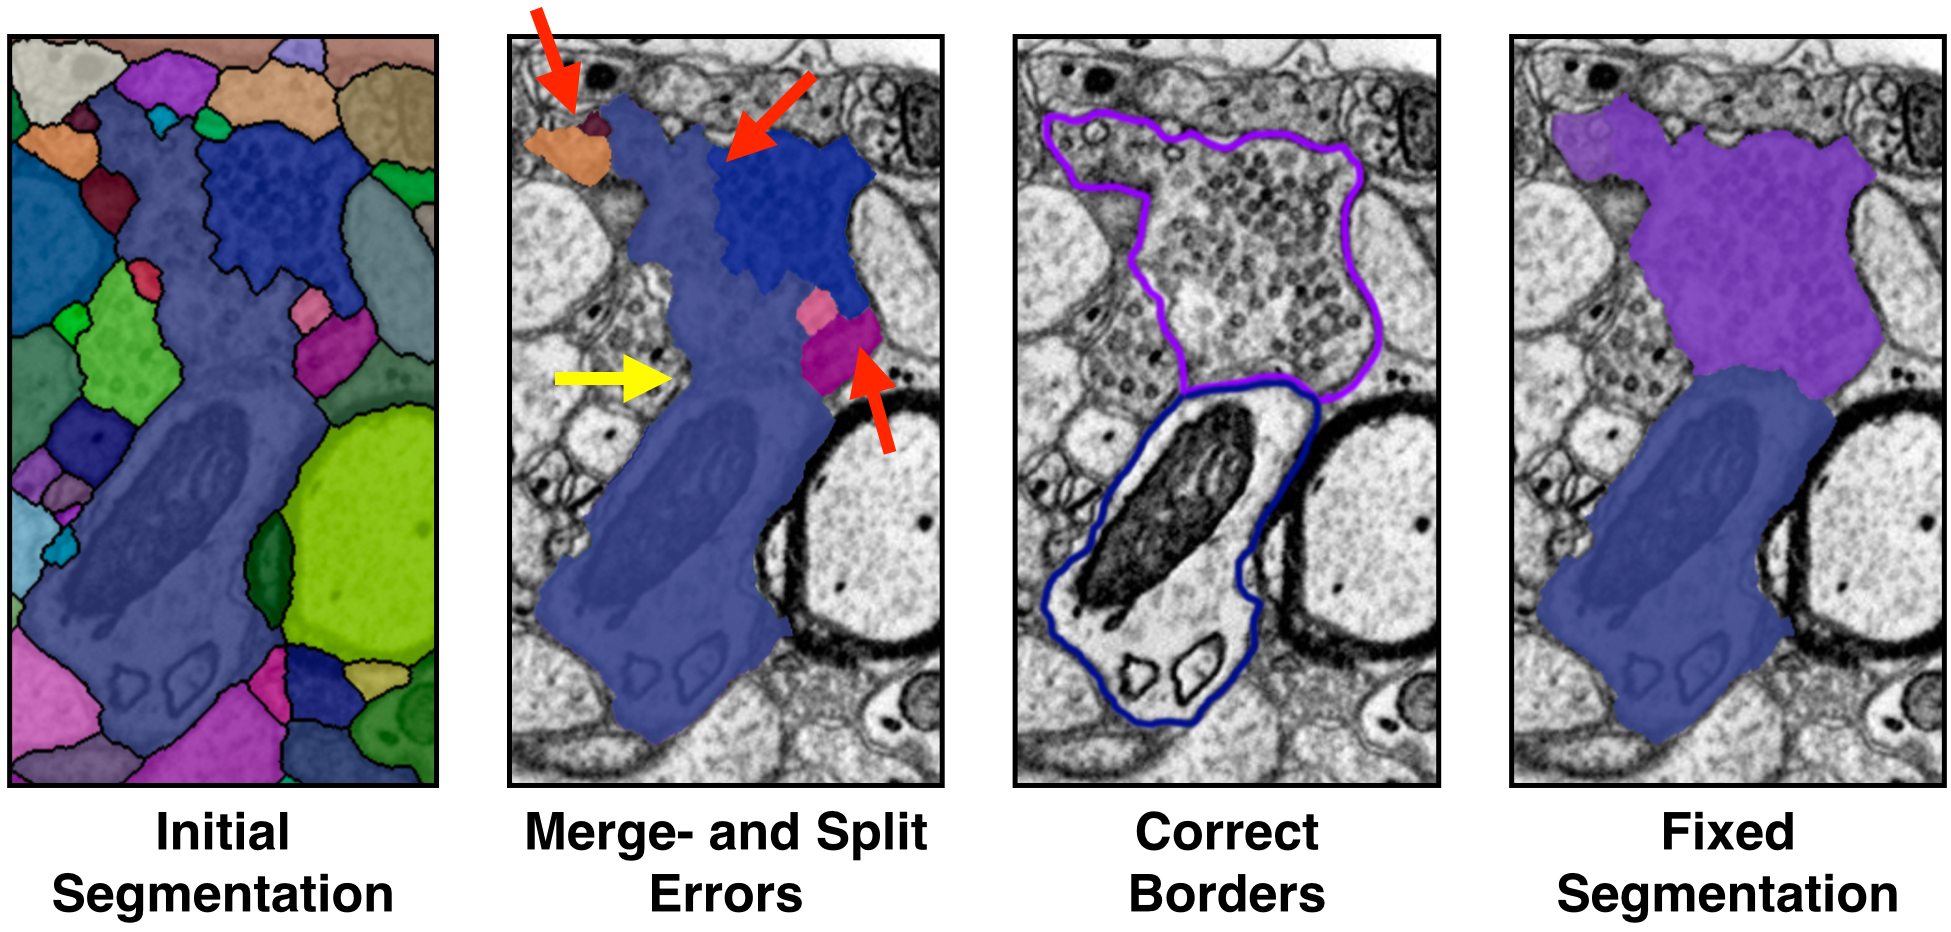
\includegraphics[width=\linewidth]{gfx/merge_and_split_errors.png}
\end{center}
\vspace{-4mm}
   \caption{The most common proofreading corrections are fixing split errors (red arrows) and merge errors (yellow arrow). A fixed segmentation matches the cell borders.}
\label{fig:merge_and_slit_errors}
\end{figure}

Our goal is to add automatic detection of split and merge errors to proofreading tools. Instead of the user visually inspecting the whole data volume carefully to spot errors, we design automatic classifiers that detect split and merge errors in 2D segmentations. Then, a proofreading tool can recommend regions with a high probability of an error to the user, and suggest corrections to accept or reject. We call this process \textit{guided proofreading} (GP).

As our main contribution, we introduce classifiers to detect merge- and split errors based on a convolutional neural network (CNN). We believe that this is the first time that deep learning is applied to the task of proofreading --- especially in the field of connectomics. Our classifiers work on top of any existing automatic segmentation method to find potential errors and suggest corrections. Given a membrane segmentation from a fast automatic method, our classifiers operate on the boundaries of whole cell regions. Compared to techniques that must analyze every input pixel, we reduce the data analysis to the boundaries only. Explicitly, we train a CNN to detect only split errors. We then reuse the same network to also detect merge errors by generating possible boundaries within a cell and inverting the split error score. Correction suggestion for both types of errors is then trivial and our technique therefor reduces the proofreading operation to simple yes/no decisions. 

We further propose a greedy algorithm to perform proofreading automatically and measure performance as the adapted Rand error which is a common metric for segmentation comparison~\cite{RAND}. 
Our system is integrated into an existing proofreading workflow for large connectomics data. For this, we also explore an active label suggestion approach in addition to the ranking obtained by guided proofreading. We quantitatively validate automatic and human-driven variations of guided proofreading on five different real-world connectomics datasets of mouse as well as fruitfly (drosophila) brain. To study the performance of novice and expert proofreaders, we perform a between-subjects experiment and ask participants to proofread a publicly available dataset. For comparison, we establish two baselines: a recently published fully interactive proofreading tool named \textit{Dojo} by Haehn~\etal~\cite{haehn_dojo_2014} and semi-automatic \textit{focused proofreading} (FP) approach by Plaza~\cite{focused_proofreading}. In all experiments, we significantly outperform both interactive proofreading as well as Plaza's method. As a consequence, we are able to provide tools to proofread segmentations more efficiently, and so better tackle large volumes of connectomics imagery.

%The reason why we work on top of an existing segmentation rather than improving the underlying technique, is to explore the error space in a non-linear way. The real world analogy would be inspecting something with a second set of eyes and different expertise.
